%%%%%%%%%%%%%%%%%%%%%%%%%%%%%%%%%%%%%%%%%%%%%%%%%%%%%%%%%%%%%%%%%%%%%%%%%%%%%%%%%%%%
% Document data
%%%%%%%%%%%%%%%%%%%%%%%%%%%%%%%%%%%%%%%%%%%%%%%%%%%%%%%%%%%%%%%%%%%%%%%%%%%%%%%%%%%%
\documentclass[12pt]{article} %report allows for chapters
%%%%%%%%%%%%%%%%%%%%%%%%%%%%%%%%%%%%%%%%%%%%%%%%%%%%%%%%%%%%%%%%%%%%%%%%%%%%%%%%%%%%
\usepackage{preamble}
\newcommand{\grad}{\boldsymbol{\vec{\nabla}}}
\newcommand{\curvegamma}{\boldsymbol{\vec{\gamma}}}
\newcommand{\tangentgamma}{\boldsymbol{\dot{\vec{\gamma}}}}
\newcommand{\vecfieldE}{\boldsymbol{\vec{E}}}
\newcommand{\rhat}{\boldsymbol{\hat{r}}}
\newcommand{\thetahat}{\boldsymbol{\hat{\theta}}}
\newcommand{\phihat}{\boldsymbol{\hat{\phi}}}
\newcommand{\unitvec}{\boldsymbol{\hat{n}}}
\newcommand{\innprod}[2]{\langle #1, #2\rangle}
\definecolor{nice_blue}{RGB}{59,140,245} 

\newcommand\boldblue[1]{\textcolor{nice_blue}{\emph{\textbf{#1}}}}
\begin{document}

\begin{center}
   \textsc{\large MATH 272, Homework 8, \emph{Solutions}}\\
   \textsc{Due April 6$^\textrm{th}$}
\end{center}
\vspace{.5cm}

\begin{problem}
	Write down the definition for a vector space.  
\end{problem}
\begin{solution}
	     A \boldblue{vector space} $V$ over a field $\mathbb{F}$ is a set of elements we call \boldblue{vectors} that satisfy the following properties. Take vectors $\vecu,\vecv,\vecw \in V$ and scalars $\alpha, \beta \in \mathbb{F}$. Then, we require that $\alpha\vecv + \beta\vecu \in V$ and 
	            \begin{enumerate}[(i)]
	                \item (Commutivity of vector addition)
	                \[
	                \vecu+\vecv=\vecv+\vecu
	                \]
	                \item (Associativity of vector addition)
	                \[
	                \vecu+(\vecv+\vecw)=(\vecu+\vecv)+\vecw;
	                \]
	                \item (Neutral element) There exists $\zerovec$ such that
	                \[
	                \zerovec+\vecv=\vecv;
	                \]
	                \item (Inverse element) For each $\vecv$ there exists $-\vecv$ such that
	                \[
	                \vecv+(-\vecv)=\zerovec;
	                \]                
	                \item (Assosciativity of scalar multiplication) We have
	                \[
	                \alpha(\beta \vecv)=(\alpha \beta)\vecv;
	                \]
	                \item (Distribution over vector addition) we have
	                \[
	                \alpha(\vecu+\vecv)=\alpha \vecu + \alpha \vecv;
	                \]
	                \item (Distribution over field addition) we have
	                \[
	                (\alpha+\beta)\vecv = \alpha \vecv + \beta \vecv;
	                \]
	                \item (Unit element) There exists $1\in \mathbb{F}$ such that
	                \[
	                1\vecv = \vecv.
	                \]
	            \end{enumerate}
\end{solution}	

\newpage
\begin{problem}
	For the following vectors in $\C^3$, compute each pairwise Hermitian inner product $\innprod{\cdot}{\cdot}$.  
	\[
		\vecu = \begin{pmatrix} i \\ 1 \\ 0 \end{pmatrix}, \qquad \vecv = \begin{pmatrix} 1 \\ -i \\ 0 \end{pmatrix}, \qquad \vecw = \begin{pmatrix} i \\ 2i \\ 2 \end{pmatrix}.
	\]
\end{problem}
\begin{solution}
	Recall that the Hermitian inner product for vectors in $\C^n$ is given by
	\[
	\innprod{\vecu}{\vecv} = \sum_{j=1}^\infty u_j v_j^*.
	\]
	So in this case, we must compute
	\[
	\innprod{\vecu}{\vecv}, \qquad \innprod{\vecu}{\vecw}, \qquad \innprod{\vecv}{\vecw}.
	\]
	Thus we have
	\begin{align*}
		\innprod{\vecu}{\vecv} &= (i)(1)^*+(1)(-i)^*+(0)(0)^*\\
			&= i +i\\
			&= 2i.
	\end{align*}
	Next,
		\begin{align*}
			\innprod{\vecu}{\vecw} &= (i)(i)^*+(1)(2i)^*+(0)(2)^*\\
				&= 1-2i.
		\end{align*}
	Finally,
	\begin{align*}
		\innprod{\vecv}{\vecw} &= (1)(i)^*+(-i)(2i)^*+(0)(2)^*\\
		&=-2-i.
	\end{align*}
\end{solution}

\newpage
\begin{problem}
	Write down what it means to have an orthonormal basis for the vector space $\R^n$ and the vector space $\C^n$.
\end{problem}
\begin{solution}~
	\begin{itemize}
		\item A basis for the vector space $\R^n$ is the smallest list of vectors so that any vector $\vecv\in \R^n$ can be written as a linear combination of the basis vectors. In this case, you will need $n$ linearly independent vectors. Moreover, the vectors in the basis (denote by $\xhat_1,\xhat_2,\dots,\xhat_n$) are normalized so that
		\[
		\|\xhat_j\|=\xhat_j \cdot \xhat_j=1,
		\]
		and orthogonal so that
		\[
		\xhat_j\cdot \xhat_k=0
		\]
		if $j\neq k$. Often one may see this condensed into the following
		\[
		\xhat_j \cdot \xhat_k = \delta_{jk},
		\]
		where $\delta_{jk}$ is the Kronecker delta which is given by
		\[
		\delta_{jk} =  \begin{cases} 0 & j\neq k \\ 1 & j=k\end{cases}.
		\]
		\item The story is analogous in $\C^n$ except that the inner product is different. Instead, we take the Hermitian inner product $\innprod{\cdot}{\cdot}$ instead of the dot product.  Thus, we will have a list of $n$ vectors $\zhat_1,\zhat_2,\dots,\zhat_n$ such that
		\[
		\innprod{\zhat_j}{\zhat_k} = \delta_{jk}.
		\]
	\end{itemize}
	The moral is that orthonormal bases depend on the space and the choice of inner product. So, we need to be careful we are aware of both when working a problem!
\end{solution}

\newpage
\begin{problem}
	(Pointwise) We often extend operations that we perform with numbers to functions without spending too much time on how this is done. For example, you know perfectly well what it means to evaluate
	\[
		5+7
	\]
	but what does it mean to evaluate
	\[
		f(x)=\cos(x)+\sin(x)?
	\]
	I'd argue that you know what this means as well.  In the above, we simply evaluate the added functions \emph{pointwise} by computing the value of each individual function at the point $x$ and then adding the resulting numbers afterwards. For example,
	\[
		f(3\pi/4)=\cos(3\pi/4) + \sin(3\pi/4)= -\frac{1}{\sqrt{2}}+\frac{1}{\sqrt{2}}=0.
	\]
	For the following, explain how the operation is to be performed on functions for some arbitrary functions $g(x)$ and $h(x)$.
	\begin{enumerate}[(a)]
		\item $g^*(x)$;
		\item $g(x)h(x)$;
		\item $(g(x))^{-1}(h^*(x))^2$.
	\end{enumerate}
\end{problem}
\begin{solution}~
	\begin{enumerate}[(a)]
		\item We will plug in a value $x$ into the function $g$ which gives us a (possibly complex) number $g(x)$. Then, we find $g^*(x)$ by taking the complex conjugate of this number $g(x)$. In other words, it may be easier to realize this as
		\[
		g^*(x)=(g(x))^*.
		\]
		\item Here, we plug in a value $x$ into both functions $g$ and $h$ to get the number values $g(x)$ and $h(x)$. Then we find $g(x)h(x)$ by multiplying the numbers we got.
		\item Take a value $x$ and plug it into the functions $g$ and $h$. Then we can take $1/g(x)=(g(x))^{-1}$. Next, we can take the complex conjugate of $h(x)$ and  then square that value to find $(h^*(x))^2$. Finally, we multiply our $(g(x))^{-1}$ by $(h^*(x))^2$.
		\end{enumerate}
\end{solution}

\newpage
\begin{problem}
	Consider the complex valued function $f(x) = \cos(x)+i\sin(x)$.  
	\begin{enumerate}[(a)]
		\item Plot this function in the complex plane for the input values $[0,2\pi]$. Clearly label the function values for $x=0,\pi/2,\pi,3\pi/2,2\pi$.
		\item Write this function in polar form. That is, find fuctions $r(x)$ and $\theta(x)$ so that $f(x)=r(x)e^{i\theta(x)}$. \emph{Hint: There are a few ways to do this, but can you use the geometry from (a) to help you here?}
		\item Evaluate the integral
		\[
			\int_0^{2\pi}f(x)dx.
		\]
		\item Evaluate the inner product for complex functions given by the integral
		\[
			\innprod{f}{f}\coloneqq \int_0^{2\pi} |f(x)|^2dx
		\]
		where $|\cdot|^2$ is the modulus squared of a complex number. You will need to realize what the modulus of a complex function is. \emph{Hint: think pointwise.}
	\end{enumerate}
\end{problem}
\begin{solution}~
	\begin{enumerate}[(a)]
		\item ~
		\begin{figure}[H]
			\centering
			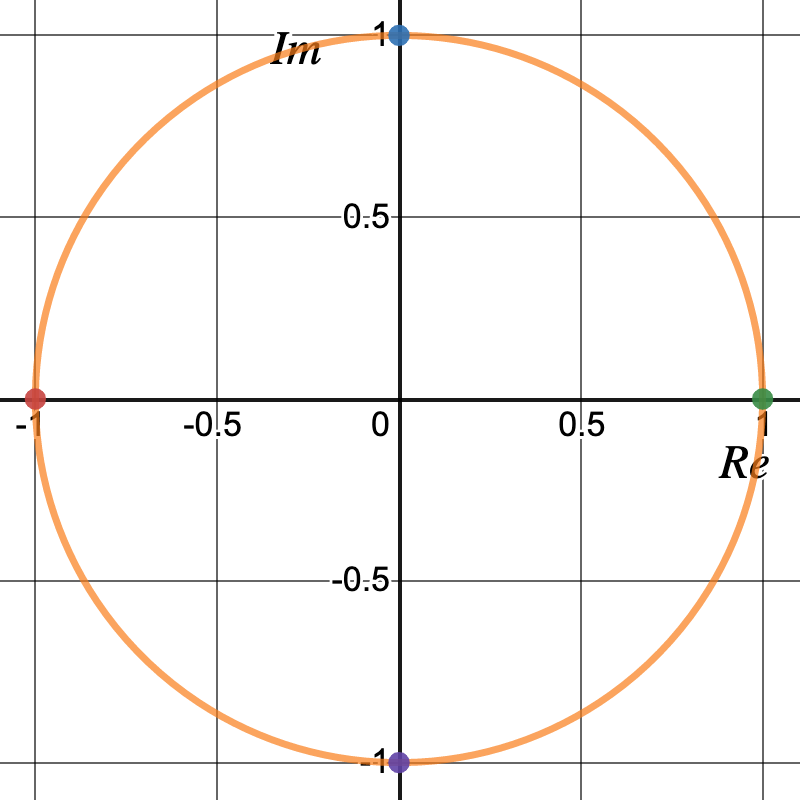
\includegraphics[width=.5\textwidth]{figures/circle_parameterization.png}
			\caption{A graph of the function $f(x)$ in orange. Green, blue, red, purple, and green dots label the output values $f(x)$ for the input values $x=0,\pi/2,\pi,3\pi/2,2\pi$ respectively.}
		\end{figure}
		\item This function is very nicely written in complex form.  Notice the outputs are all on the unit circle, and thus $r(x)=1$.  We can also see this by noting 
		\[
		\|\cos(x)+i\sin(x)\|=1,
		\]
		since $\sin^2(x)+\cos^2(x)=1$.  We could also realize this from Euler's formula in that
		\[
		r(x)e^{i\theta(x)}=r(x)\cos(\theta(x))+ir(x)\sin(\theta(x)).
		\]
		Euler's formula then shows us that we must also have $\theta(x)=x$. Hence, in polar form, our function is given by
		\[
		f(x)=e^{ix}.
		\]
		\item We compute this in the same way as any integral we have done before. We have
		\begin{align*}
			\int_0^{2\pi} f(x) dx &= \int_0^{2\pi} e^{ix}dx\\
			&= \left. \frac{1}{i} e^{ix} \right\vert_0^{2\pi}\\
			&= 0.
		\end{align*}
		\item Now we know that $\|f(x)\|^2=1$ by the work in (a). Hence, we simply have
		\begin{align*}
			\int_0^{2\pi} 1 dx &= x\vert_0^{2\pi}\\
			&= 2\pi
		\end{align*}
		This just so happens to be the circumference of the circle.  
	\end{enumerate}
\end{solution}


\end{document}